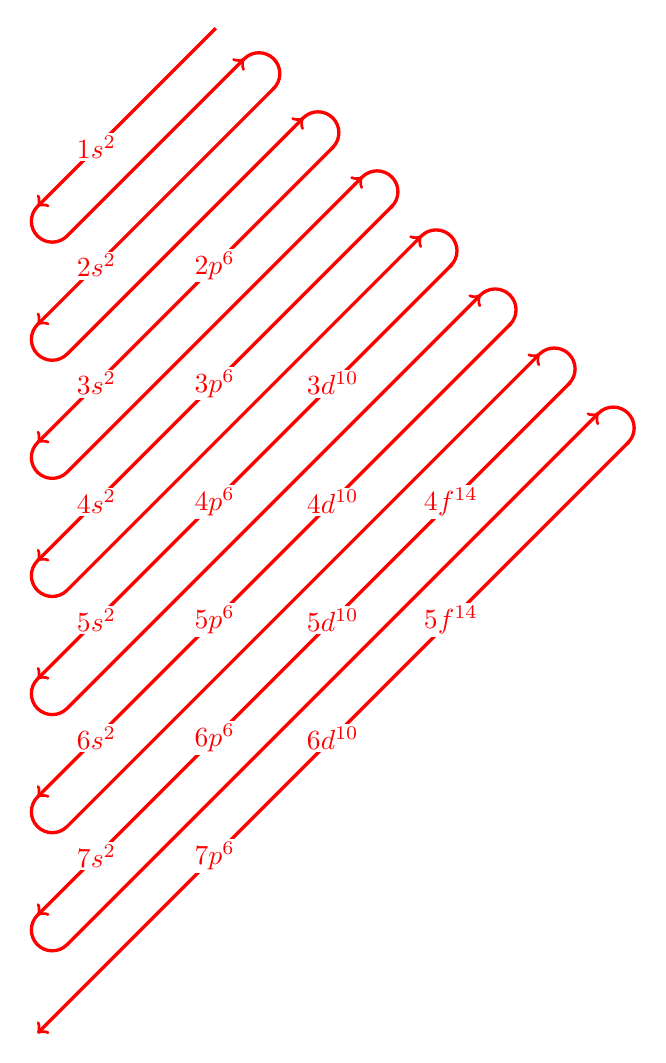
\begin{tikzpicture}[scale=1.5, y={(0cm,-1cm)}, line cap=rect]
        \foreach\y in {1,...,8}
        {%
        \ifnum\y > 1
            \draw[very thick, red]    (0.5*\y+1.25,0.5*\y-0.75) arc (-135:45:{0.125*sqrt(2)});
        \fi
        \draw[very thick,->, red]   (0.5*\y+1.5,0.5*\y-0.5) -- (0.5,\y+0.5);
        \ifnum \y < 8
            \draw[very thick,->, red] (0.5,\y+0.5) arc (225:45:{0.125*sqrt(2)}) --
            (0.5*\y+1.75,0.5*\y-0.25);
        \fi
        }
        \foreach\y in {1,...,7}
            {%
                \pgfmathtruncatemacro\maxx{6-abs(4.5-\y)}
                \foreach[count=\x]\i in {s,p,d,f}
                    {%
                        \ifnum \x < \maxx
                            \pgfmathtruncatemacro\ne{2*(2*\x-1)}
                            \node[fill=white, text=red, inner sep=1pt] at (\x,\y) {$\y\i^{\ne}$};
                        \fi
                    }
            }
\end{tikzpicture}